
\chapter{}\label{ch:auf2}
In dieser Aufgabe sind die Signale der Hallsensoren, sowie die idealisierten Stromverläufe des BLDC im Linkslauf gegeben.

\section{}\label{sec:2a}
\textit{Skizzieren Sie die entsprechenden Signale der Hallsensoren und die idealisierten Stromverläufe bei Rechtslauf.}\\
In den Abbildungen \ref{fig:2a:hall} und \ref{fig:2a:strom} kann man die Hallsensorsignale erkennen, sowie die dazugehörigen Stromverläufe der jeweiligen Wicklungen U,V und W. Sie sind hier im Rechtslauf dargestellt. Wenn man die Motorwelle von vorne betrachtet, dann sieht man, dass sie sich im Rechtslauf befindet (dies bedeutet, er dreht sich im Uhrzeigersinn). Wenn sich der Motor im linkslauf befindet, so dreht dieser sich gegen den Uhrzeigersinn.
\begin{figure}[h]
	\centering
	% This file was created by matlab2tikz.
%
%The latest updates can be retrieved from
%  http://www.mathworks.com/matlabcentral/fileexchange/22022-matlab2tikz-matlab2tikz
%where you can also make suggestions and rate matlab2tikz.
%
\definecolor{mycolor1}{rgb}{0.00000,0.44700,0.74100}%
\definecolor{mycolor2}{rgb}{0.85000,0.32500,0.09800}%
\definecolor{mycolor3}{rgb}{0.92900,0.69400,0.12500}%
%
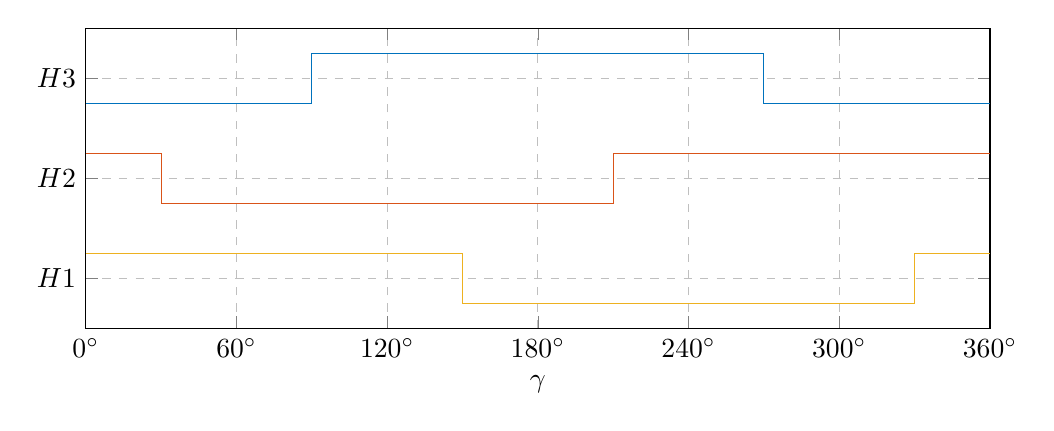
\begin{tikzpicture}

\begin{axis}[%
width=4.521in,
height=1.5in,
at={(0.758in,0.481in)},
scale only axis,
xmin=0,
xmax=360,
xtick={ 0,  60, 120, 180, 240, 300, 360},
xticklabels={{$ 0^{\circ} $},  {$ 60^{\circ} $}, {$ 120^{\circ} $}, {$ 180^{\circ} $}, {$ 240^{\circ} $}, {$ 300^{\circ} $}, {$ 360^{\circ} $}},
xlabel={$\gamma$},
ymin=-1,
ymax=11,
ytick={1,5,9},
yticklabels={{$ H1 $},{$ H2 $},{$ H3 $}},
axis background/.style={fill=white},
xmajorgrids,
ymajorgrids,
major grid style={dashed}
]
\addplot[const plot, color=mycolor1, forget plot] table[row sep=crcr] {%
0	8\\
30	8\\
60	8\\
90	10\\
120	10\\
150	10\\
180	10\\
210	10\\
240	10\\
270	8\\
300	8\\
330	8\\
360	8\\
};
\addplot[const plot, color=mycolor2, forget plot] table[row sep=crcr] {%
0	6\\
30	4\\
60	4\\
90	4\\
120	4\\
150	4\\
180	4\\
210	6\\
240	6\\
270	6\\
300	6\\
330	6\\
360	6\\
};
\addplot[const plot, color=mycolor3, forget plot] table[row sep=crcr] {%
0	2\\
30	2\\
60	2\\
90	2\\
120	2\\
150	0\\
180	0\\
210	0\\
240	0\\
270	0\\
300	0\\
330	2\\
360	2\\
};
\end{axis}
\end{tikzpicture}%
	\caption{Signale der Hallsensoren im Rechtslauf}
	\label{fig:2a:hall}
\end{figure}
\begin{figure}[h]
	\centering
	% This file was created by matlab2tikz.
%
%The latest updates can be retrieved from
%  http://www.mathworks.com/matlabcentral/fileexchange/22022-matlab2tikz-matlab2tikz
%where you can also make suggestions and rate matlab2tikz.
%
\definecolor{mycolor1}{rgb}{0.00000,0.44700,0.74100}%
\definecolor{mycolor2}{rgb}{0.85000,0.32500,0.09800}%
\definecolor{mycolor3}{rgb}{0.92900,0.69400,0.12500}%
%
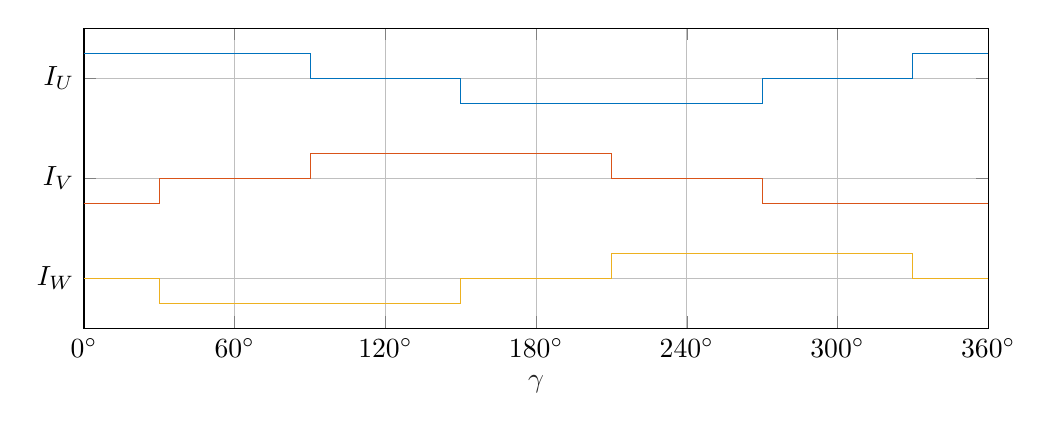
\begin{tikzpicture}

\begin{axis}[%
width=4.521in,
height=1.5in,
at={(0.758in,0.481in)},
scale only axis,
xmin=0,
xmax=360,
xtick={ 0,  60, 120, 180, 240, 300, 360},
xticklabels={{$ 0^{\circ} $},  {$ 60^{\circ} $}, {$ 120^{\circ} $}, {$ 180^{\circ} $}, {$ 240^{\circ} $}, {$ 300^{\circ} $}, {$ 360^{\circ} $}},
xlabel style={font=\color{white!15!black}},
xlabel={$\gamma$},
ymin=-1,
ymax=11,
ytick={1,5,9},
yticklabels={{$ I_{W} $},{$ I_{V} $},{$ I_{U} $}},
axis background/.style={fill=white},
xmajorgrids,
ymajorgrids
]
\addplot[const plot, color=mycolor1, forget plot] table[row sep=crcr] {%
0	10\\
30	10\\
60	10\\
90	9\\
120	9\\
150	8\\
180	8\\
210	8\\
240	8\\
270	9\\
300	9\\
330	10\\
360	10\\
};
\addplot[const plot, color=mycolor2, forget plot] table[row sep=crcr] {%
0	4\\
30	5\\
60	5\\
90	6\\
120	6\\
150	6\\
180	6\\
210	5\\
240	5\\
270	4\\
300	4\\
330	4\\
360	4\\
};
\addplot[const plot, color=mycolor3, forget plot] table[row sep=crcr] {%
0	1\\
30	0\\
60	0\\
90	0\\
120	0\\
150	1\\
180	1\\
210	2\\
240	2\\
270	2\\
300	2\\
330	1\\
360	1\\
};
\end{axis}
\end{tikzpicture}%
	\caption{Stromverläufe im Rechtslauf}
	\label{fig:2a:strom}
\end{figure}

\section{}\label{sec:2b}
In diesem Aufgabenteil sollen nun zu den rechtsläufigen Stromverläufen aus Aufgabenteil a) die entsprechenden binären Ansteuersignale der sechs Transistoren in einem Diagramm dargestellt werden. Ist der Transistor leitend, so entspricht dies einem positiven Ansteuersignal mit dem Wert 1. Wenn der Transistor sperrt, so entspricht dies dem binären Wert 0. Abbildung \ref{fig:2b:rechts} zeigt die Ansteuerung der sechs Transistoren für den Stromverlauf.
\begin{figure}[h]
	\centering
	% This file was created by matlab2tikz.
%
%The latest updates can be retrieved from
%  http://www.mathworks.com/matlabcentral/fileexchange/22022-matlab2tikz-matlab2tikz
%where you can also make suggestions and rate matlab2tikz.
%
\definecolor{mycolor1}{rgb}{0.00000,0.44700,0.74100}%
\definecolor{mycolor2}{rgb}{0.85000,0.32500,0.09800}%
\definecolor{mycolor3}{rgb}{0.92900,0.69400,0.12500}%
\definecolor{mycolor4}{rgb}{0.49400,0.18400,0.55600}%
\definecolor{mycolor5}{rgb}{0.46600,0.67400,0.18800}%
\definecolor{mycolor6}{rgb}{0.30100,0.74500,0.93300}%
%
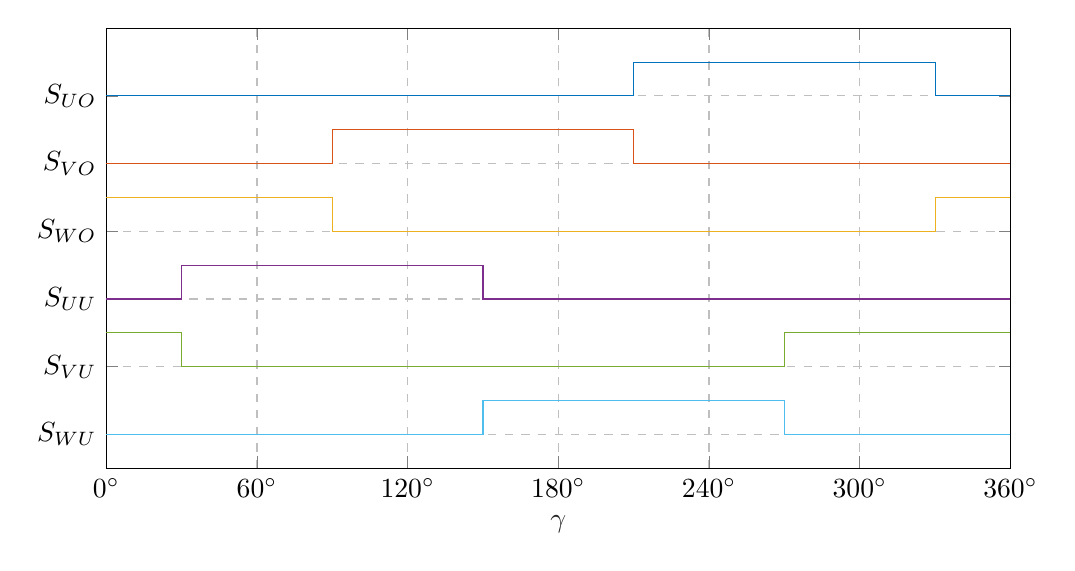
\begin{tikzpicture}

\begin{axis}[%
width=4.521in,
height=2.2in,
at={(0.758in,0.481in)},
scale only axis,
xmin=0,
xmax=360,
xtick={ 0,  60, 120, 180, 240, 300, 360},
xticklabels={{$ 0^{\circ} $},  {$ 60^{\circ} $}, {$ 120^{\circ} $}, {$ 180^{\circ} $}, {$ 240^{\circ} $}, {$ 300^{\circ} $}, {$ 360^{\circ} $}},
xlabel style={font=\color{white!15!black}},
xlabel={$\gamma$},
ymin=-1,
ymax=12,
ytick={0,2,4,6,8,10},
yticklabels={{$ S_{WU} $},{$ S_{VU} $},{$ S_{UU} $},{$ S_{WO} $},{$ S_{VO}$},{$ S_{UO} $}},
axis background/.style={fill=white},
%axis x line*=bottom,
%axis y line*=left,
xmajorgrids,
ymajorgrids,
major grid style={dashed}
]
\addplot[const plot, color=mycolor1, forget plot] table[row sep=crcr] {%
0	10\\
30	10\\
60	10\\
90	10\\
120	10\\
150	10\\
180	10\\
210	11\\
240	11\\
270	11\\
300	11\\
330	10\\
360	10\\
};
\addplot[const plot, color=mycolor2, forget plot] table[row sep=crcr] {%
0	8\\
30	8\\
60	8\\
90	9\\
120	9\\
150	9\\
180	9\\
210	8\\
240	8\\
270	8\\
300	8\\
330	8\\
360	8\\
};
\addplot[const plot, color=mycolor3, forget plot] table[row sep=crcr] {%
0	7\\
30	7\\
60	7\\
90	6\\
120	6\\
150	6\\
180	6\\
210	6\\
240	6\\
270	6\\
300	6\\
330	7\\
360	7\\
};
\addplot[const plot, color=mycolor4, forget plot] table[row sep=crcr] {%
0	4\\
30	5\\
60	5\\
90	5\\
120	5\\
150	4\\
180	4\\
210	4\\
240	4\\
270	4\\
300	4\\
330	4\\
360	4\\
};
\addplot[const plot, color=mycolor5, forget plot] table[row sep=crcr] {%
0	3\\
30	2\\
60	2\\
90	2\\
120	2\\
150	2\\
180	2\\
210	2\\
240	2\\
270	3\\
300	3\\
330	3\\
360	3\\
};
\addplot[const plot, color=mycolor6, forget plot] table[row sep=crcr] {%
0	0\\
30	0\\
60	0\\
90	0\\
120	0\\
150	1\\
180	1\\
210	1\\
240	1\\
270	0\\
300	0\\
330	0\\
360	0\\
};
\end{axis}
\end{tikzpicture}%
	\caption{Ansteuersignale im Rechtslauf}
	\label{fig:2b:rechts}
\end{figure}

\section{}\label{sec:2c}
Für den Linkslauf des BLDCs sollen jetzt die Ansteuersignale geändert werden.
Damit der Motor in den Linkslauf wechselt, müssen jeweils die Steuersignale zweier Transistoren eines Strangs miteinander getauscht werden: $ S_{VO} $ + $ S_{UU} $, $ S_{VO} $ + $ S_{VU} $ und $ S_{WO} $ + $ S_{WU} $. Dieser Tausch ist in Abbildung \ref{fig:2b:links} nachzuvollziehen.
\begin{figure}[h]
	\centering
	% This file was created by matlab2tikz.
%
%The latest updates can be retrieved from
%  http://www.mathworks.com/matlabcentral/fileexchange/22022-matlab2tikz-matlab2tikz
%where you can also make suggestions and rate matlab2tikz.
%
\definecolor{mycolor1}{rgb}{0.00000,0.44700,0.74100}%
\definecolor{mycolor2}{rgb}{0.85000,0.32500,0.09800}%
\definecolor{mycolor3}{rgb}{0.92900,0.69400,0.12500}%
\definecolor{mycolor4}{rgb}{0.49400,0.18400,0.55600}%
\definecolor{mycolor5}{rgb}{0.46600,0.67400,0.18800}%
\definecolor{mycolor6}{rgb}{0.30100,0.74500,0.93300}%
%
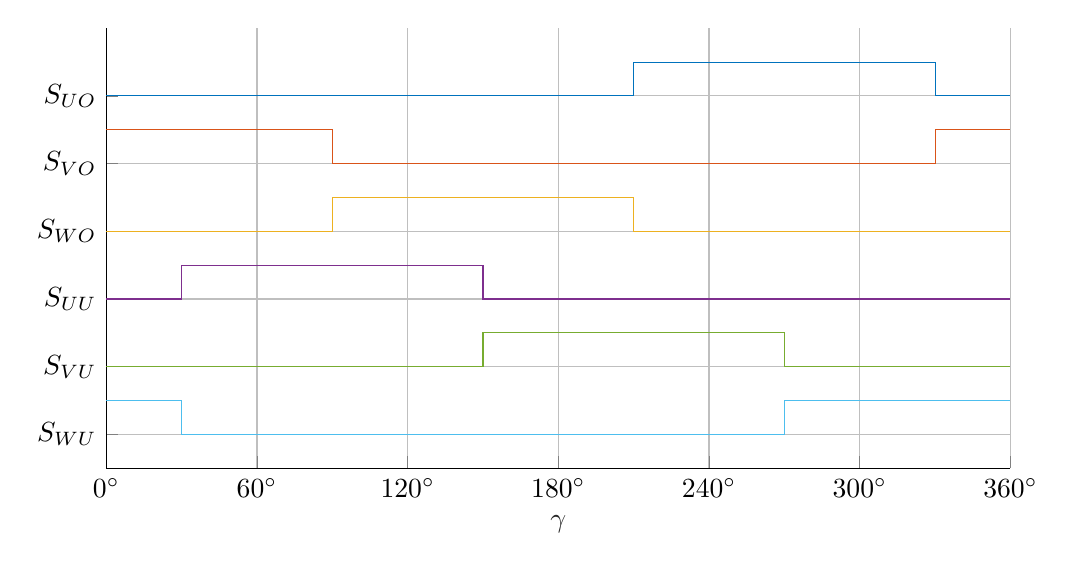
\begin{tikzpicture}

\begin{axis}[%
width=4.521in,
height=2.2in,
at={(0.758in,0.481in)},
scale only axis,
xmin=0,
xmax=360,
xtick={  0,  60, 120, 180, 240, 300, 360},
xticklabels={{$ 0^{\circ} $},  {$ 60^{\circ} $}, {$ 120^{\circ} $}, {$ 180^{\circ} $}, {$ 240^{\circ} $}, {$ 300^{\circ} $}, {$ 360^{\circ} $}},
xlabel style={font=\color{white!15!black}},
xlabel={$\gamma$},
ymin=-1,
ymax=12,
ytick={0,2,4,6,8,10},
yticklabels={{$ S_{WU} $},{$ S_{VU} $},{$ S_{UU} $},{$ S_{WO} $},{$ S_{VO}$},{$ S_{UO} $}},
axis background/.style={fill=white},
axis x line*=bottom,
axis y line*=left,
xmajorgrids,
ymajorgrids
]
\addplot[const plot, color=mycolor1, forget plot] table[row sep=crcr] {%
0	10\\
30	10\\
60	10\\
90	10\\
120	10\\
150	10\\
180	10\\
210	11\\
240	11\\
270	11\\
300	11\\
330	10\\
360	10\\
};
\addplot[const plot, color=mycolor2, forget plot] table[row sep=crcr] {%
0	9\\
30	9\\
60	9\\
90	8\\
120	8\\
150	8\\
180	8\\
210	8\\
240	8\\
270	8\\
300	8\\
330	9\\
360	9\\
};
\addplot[const plot, color=mycolor3, forget plot] table[row sep=crcr] {%
0	6\\
30	6\\
60	6\\
90	7\\
120	7\\
150	7\\
180	7\\
210	6\\
240	6\\
270	6\\
300	6\\
330	6\\
360	6\\
};
\addplot[const plot, color=mycolor4, forget plot] table[row sep=crcr] {%
0	4\\
30	5\\
60	5\\
90	5\\
120	5\\
150	4\\
180	4\\
210	4\\
240	4\\
270	4\\
300	4\\
330	4\\
360	4\\
};
\addplot[const plot, color=mycolor5, forget plot] table[row sep=crcr] {%
0	2\\
30	2\\
60	2\\
90	2\\
120	2\\
150	3\\
180	3\\
210	3\\
240	3\\
270	2\\
300	2\\
330	2\\
360	2\\
};
\addplot[const plot, color=mycolor6, forget plot] table[row sep=crcr] {%
0	1\\
30	0\\
60	0\\
90	0\\
120	0\\
150	0\\
180	0\\
210	0\\
240	0\\
270	1\\
300	1\\
330	1\\
360	1\\
};
\end{axis}
\end{tikzpicture}%
	\caption{Ansteuersignale im Linkslauf}
	\label{fig:2b:links}
\end{figure}

\section{}\label{sec:2d}
Für den unseren BLDC sind folgende Parameter gegeben:
\begin{center}
	 $ R_{AP} = 0,8\Omega $ und $ L_{AP} = 1,1mH$\\
\end{center}
Es soll nun für den Spannungsverlauf $ U_{U} $ der Verlauf des Ankerstroms im Strang $ U $ skizziert werden, siehe Abbildung \ref{fig:2d:strom}. Für die Berechnung nehmen wir an, dass die innere Spannung gleich Null ist.\\
Für die Berechnung der Zeitkonstante benutzen wir diese Formel:\\
\begin{equation}
	\tau = \frac{L_{AP}}{R_{AP}} = \frac{1,1mH}{0,8\Omega} = 1,375ms
\end{equation}
Den maximalen Strangstrom berechnen wir wie folgt:
\begin{equation}
	I_{max} = \frac{U_{U}}{R_{LAP}} = \frac{12V}{0,8\Omega} = 15A
\end{equation}
\begin{figure}[h]
	\centering
	% This file was created by matlab2tikz.
%
%The latest updates can be retrieved from
%  http://www.mathworks.com/matlabcentral/fileexchange/22022-matlab2tikz-matlab2tikz
%where you can also make suggestions and rate matlab2tikz.
%
\definecolor{mycolor1}{rgb}{0.00000,0.44700,0.74100}%
\definecolor{mycolor2}{rgb}{0.85000,0.32500,0.09800}%
%
\begin{tikzpicture}

\begin{axis}[%
compat=1.3,
width=4.521in,
height=3.566in,
at={(0.758in,0.481in)},
scale only axis,
xmin=-1,
xmax=10,
xtick={ 0,  2,  4,  6,  8, 10},
separate axis lines,
every outer y axis line/.append style={mycolor2},
every y tick label/.append style={font=\color{mycolor2}},
every y tick/.append style={mycolor2},
ymin=0,
ymax=18.75,
ytick={ 0,  3,  6,  9, 12, 15},
ylabel style={font=\color{mycolor2}},
ylabel={IU/A},
axis background/.style={fill=white},
yticklabel pos=right,
xmajorgrids,
ymajorgrids,
major grid style={dashed}
]
\addplot [color=mycolor1, forget plot]
  table[row sep=crcr]{%
-1	0\\
-0.99	0\\
-0.98	0\\
-0.97	0\\
-0.96	0\\
-0.95	0\\
-0.94	0\\
-0.93	0\\
-0.92	0\\
-0.91	0\\
-0.9	0\\
-0.89	0\\
-0.88	0\\
-0.87	0\\
-0.86	0\\
-0.85	0\\
-0.84	0\\
-0.83	0\\
-0.82	0\\
-0.81	0\\
-0.8	0\\
-0.79	0\\
-0.78	0\\
-0.77	0\\
-0.76	0\\
-0.75	0\\
-0.74	0\\
-0.73	0\\
-0.72	0\\
-0.71	0\\
-0.7	0\\
-0.69	0\\
-0.68	0\\
-0.67	0\\
-0.66	0\\
-0.65	0\\
-0.64	0\\
-0.63	0\\
-0.62	0\\
-0.61	0\\
-0.6	0\\
-0.59	0\\
-0.58	0\\
-0.57	0\\
-0.56	0\\
-0.55	0\\
-0.54	0\\
-0.53	0\\
-0.52	0\\
-0.51	0\\
-0.5	0\\
-0.49	0\\
-0.48	0\\
-0.47	0\\
-0.46	0\\
-0.45	0\\
-0.44	0\\
-0.43	0\\
-0.42	0\\
-0.41	0\\
-0.4	0\\
-0.39	0\\
-0.38	0\\
-0.37	0\\
-0.36	0\\
-0.35	0\\
-0.34	0\\
-0.33	0\\
-0.32	0\\
-0.31	0\\
-0.3	0\\
-0.29	0\\
-0.28	0\\
-0.27	0\\
-0.26	0\\
-0.25	0\\
-0.24	0\\
-0.23	0\\
-0.22	0\\
-0.21	0\\
-0.2	0\\
-0.19	0\\
-0.18	0\\
-0.17	0\\
-0.16	0\\
-0.15	0\\
-0.14	0\\
-0.13	0\\
-0.12	0\\
-0.11	0\\
-0.1	0\\
-0.09	0\\
-0.08	0\\
-0.07	0\\
-0.0599999999999999	0\\
-0.0499999999999999	0\\
-0.04	0\\
-0.03	0\\
-0.02	0\\
-0.01	0\\
0	6\\
0.01	12\\
0.02	12\\
0.03	12\\
0.04	12\\
0.05	12\\
0.0600000000000001	12\\
0.0700000000000001	12\\
0.0800000000000001	12\\
0.0900000000000001	12\\
0.1	12\\
0.11	12\\
0.12	12\\
0.13	12\\
0.14	12\\
0.15	12\\
0.16	12\\
0.17	12\\
0.18	12\\
0.19	12\\
0.2	12\\
0.21	12\\
0.22	12\\
0.23	12\\
0.24	12\\
0.25	12\\
0.26	12\\
0.27	12\\
0.28	12\\
0.29	12\\
0.3	12\\
0.31	12\\
0.32	12\\
0.33	12\\
0.34	12\\
0.35	12\\
0.36	12\\
0.37	12\\
0.38	12\\
0.39	12\\
0.4	12\\
0.41	12\\
0.42	12\\
0.43	12\\
0.44	12\\
0.45	12\\
0.46	12\\
0.47	12\\
0.48	12\\
0.49	12\\
0.5	12\\
0.51	12\\
0.52	12\\
0.53	12\\
0.54	12\\
0.55	12\\
0.56	12\\
0.57	12\\
0.58	12\\
0.59	12\\
0.6	12\\
0.61	12\\
0.62	12\\
0.63	12\\
0.64	12\\
0.65	12\\
0.66	12\\
0.67	12\\
0.68	12\\
0.69	12\\
0.7	12\\
0.71	12\\
0.72	12\\
0.73	12\\
0.74	12\\
0.75	12\\
0.76	12\\
0.77	12\\
0.78	12\\
0.79	12\\
0.8	12\\
0.81	12\\
0.82	12\\
0.83	12\\
0.84	12\\
0.85	12\\
0.86	12\\
0.87	12\\
0.88	12\\
0.89	12\\
0.9	12\\
0.91	12\\
0.92	12\\
0.93	12\\
0.94	12\\
0.95	12\\
0.96	12\\
0.97	12\\
0.98	12\\
0.99	12\\
1	12\\
1.01	12\\
1.02	12\\
1.03	12\\
1.04	12\\
1.05	12\\
1.06	12\\
1.07	12\\
1.08	12\\
1.09	12\\
1.1	12\\
1.11	12\\
1.12	12\\
1.13	12\\
1.14	12\\
1.15	12\\
1.16	12\\
1.17	12\\
1.18	12\\
1.19	12\\
1.2	12\\
1.21	12\\
1.22	12\\
1.23	12\\
1.24	12\\
1.25	12\\
1.26	12\\
1.27	12\\
1.28	12\\
1.29	12\\
1.3	12\\
1.31	12\\
1.32	12\\
1.33	12\\
1.34	12\\
1.35	12\\
1.36	12\\
1.37	12\\
1.38	12\\
1.39	12\\
1.4	12\\
1.41	12\\
1.42	12\\
1.43	12\\
1.44	12\\
1.45	12\\
1.46	12\\
1.47	12\\
1.48	12\\
1.49	12\\
1.5	12\\
1.51	12\\
1.52	12\\
1.53	12\\
1.54	12\\
1.55	12\\
1.56	12\\
1.57	12\\
1.58	12\\
1.59	12\\
1.6	12\\
1.61	12\\
1.62	12\\
1.63	12\\
1.64	12\\
1.65	12\\
1.66	12\\
1.67	12\\
1.68	12\\
1.69	12\\
1.7	12\\
1.71	12\\
1.72	12\\
1.73	12\\
1.74	12\\
1.75	12\\
1.76	12\\
1.77	12\\
1.78	12\\
1.79	12\\
1.8	12\\
1.81	12\\
1.82	12\\
1.83	12\\
1.84	12\\
1.85	12\\
1.86	12\\
1.87	12\\
1.88	12\\
1.89	12\\
1.9	12\\
1.91	12\\
1.92	12\\
1.93	12\\
1.94	12\\
1.95	12\\
1.96	12\\
1.97	12\\
1.98	12\\
1.99	12\\
2	12\\
2.01	12\\
2.02	12\\
2.03	12\\
2.04	12\\
2.05	12\\
2.06	12\\
2.07	12\\
2.08	12\\
2.09	12\\
2.1	12\\
2.11	12\\
2.12	12\\
2.13	12\\
2.14	12\\
2.15	12\\
2.16	12\\
2.17	12\\
2.18	12\\
2.19	12\\
2.2	12\\
2.21	12\\
2.22	12\\
2.23	12\\
2.24	12\\
2.25	12\\
2.26	12\\
2.27	12\\
2.28	12\\
2.29	12\\
2.3	12\\
2.31	12\\
2.32	12\\
2.33	12\\
2.34	12\\
2.35	12\\
2.36	12\\
2.37	12\\
2.38	12\\
2.39	12\\
2.4	12\\
2.41	12\\
2.42	12\\
2.43	12\\
2.44	12\\
2.45	12\\
2.46	12\\
2.47	12\\
2.48	12\\
2.49	12\\
2.5	12\\
2.51	12\\
2.52	12\\
2.53	12\\
2.54	12\\
2.55	12\\
2.56	12\\
2.57	12\\
2.58	12\\
2.59	12\\
2.6	12\\
2.61	12\\
2.62	12\\
2.63	12\\
2.64	12\\
2.65	12\\
2.66	12\\
2.67	12\\
2.68	12\\
2.69	12\\
2.7	12\\
2.71	12\\
2.72	12\\
2.73	12\\
2.74	12\\
2.75	12\\
2.76	12\\
2.77	12\\
2.78	12\\
2.79	12\\
2.8	12\\
2.81	12\\
2.82	12\\
2.83	12\\
2.84	12\\
2.85	12\\
2.86	12\\
2.87	12\\
2.88	12\\
2.89	12\\
2.9	12\\
2.91	12\\
2.92	12\\
2.93	12\\
2.94	12\\
2.95	12\\
2.96	12\\
2.97	12\\
2.98	12\\
2.99	12\\
3	12\\
3.01	12\\
3.02	12\\
3.03	12\\
3.04	12\\
3.05	12\\
3.06	12\\
3.07	12\\
3.08	12\\
3.09	12\\
3.1	12\\
3.11	12\\
3.12	12\\
3.13	12\\
3.14	12\\
3.15	12\\
3.16	12\\
3.17	12\\
3.18	12\\
3.19	12\\
3.2	12\\
3.21	12\\
3.22	12\\
3.23	12\\
3.24	12\\
3.25	12\\
3.26	12\\
3.27	12\\
3.28	12\\
3.29	12\\
3.3	12\\
3.31	12\\
3.32	12\\
3.33	12\\
3.34	12\\
3.35	12\\
3.36	12\\
3.37	12\\
3.38	12\\
3.39	12\\
3.4	12\\
3.41	12\\
3.42	12\\
3.43	12\\
3.44	12\\
3.45	12\\
3.46	12\\
3.47	12\\
3.48	12\\
3.49	12\\
3.5	12\\
3.51	12\\
3.52	12\\
3.53	12\\
3.54	12\\
3.55	12\\
3.56	12\\
3.57	12\\
3.58	12\\
3.59	12\\
3.6	12\\
3.61	12\\
3.62	12\\
3.63	12\\
3.64	12\\
3.65	12\\
3.66	12\\
3.67	12\\
3.68	12\\
3.69	12\\
3.7	12\\
3.71	12\\
3.72	12\\
3.73	12\\
3.74	12\\
3.75	12\\
3.76	12\\
3.77	12\\
3.78	12\\
3.79	12\\
3.8	12\\
3.81	12\\
3.82	12\\
3.83	12\\
3.84	12\\
3.85	12\\
3.86	12\\
3.87	12\\
3.88	12\\
3.89	12\\
3.9	12\\
3.91	12\\
3.92	12\\
3.93	12\\
3.94	12\\
3.95	12\\
3.96	12\\
3.97	12\\
3.98	12\\
3.99	12\\
4	12\\
4.01	12\\
4.02	12\\
4.03	12\\
4.04	12\\
4.05	12\\
4.06	12\\
4.07	12\\
4.08	12\\
4.09	12\\
4.1	12\\
4.11	12\\
4.12	12\\
4.13	12\\
4.14	12\\
4.15	12\\
4.16	12\\
4.17	12\\
4.18	12\\
4.19	12\\
4.2	12\\
4.21	12\\
4.22	12\\
4.23	12\\
4.24	12\\
4.25	12\\
4.26	12\\
4.27	12\\
4.28	12\\
4.29	12\\
4.3	12\\
4.31	12\\
4.32	12\\
4.33	12\\
4.34	12\\
4.35	12\\
4.36	12\\
4.37	12\\
4.38	12\\
4.39	12\\
4.4	12\\
4.41	12\\
4.42	12\\
4.43	12\\
4.44	12\\
4.45	12\\
4.46	12\\
4.47	12\\
4.48	12\\
4.49	12\\
4.5	12\\
4.51	12\\
4.52	12\\
4.53	12\\
4.54	12\\
4.55	12\\
4.56	12\\
4.57	12\\
4.58	12\\
4.59	12\\
4.6	12\\
4.61	12\\
4.62	12\\
4.63	12\\
4.64	12\\
4.65	12\\
4.66	12\\
4.67	12\\
4.68	12\\
4.69	12\\
4.7	12\\
4.71	12\\
4.72	12\\
4.73	12\\
4.74	12\\
4.75	12\\
4.76	12\\
4.77	12\\
4.78	12\\
4.79	12\\
4.8	12\\
4.81	12\\
4.82	12\\
4.83	12\\
4.84	12\\
4.85	12\\
4.86	12\\
4.87	12\\
4.88	12\\
4.89	12\\
4.9	12\\
4.91	12\\
4.92	12\\
4.93	12\\
4.94	12\\
4.95	12\\
4.96	12\\
4.97	12\\
4.98	12\\
4.99	12\\
5	12\\
5.01	12\\
5.02	12\\
5.03	12\\
5.04	12\\
5.05	12\\
5.06	12\\
5.07	12\\
5.08	12\\
5.09	12\\
5.1	12\\
5.11	12\\
5.12	12\\
5.13	12\\
5.14	12\\
5.15	12\\
5.16	12\\
5.17	12\\
5.18	12\\
5.19	12\\
5.2	12\\
5.21	12\\
5.22	12\\
5.23	12\\
5.24	12\\
5.25	12\\
5.26	12\\
5.27	12\\
5.28	12\\
5.29	12\\
5.3	12\\
5.31	12\\
5.32	12\\
5.33	12\\
5.34	12\\
5.35	12\\
5.36	12\\
5.37	12\\
5.38	12\\
5.39	12\\
5.4	12\\
5.41	12\\
5.42	12\\
5.43	12\\
5.44	12\\
5.45	12\\
5.46	12\\
5.47	12\\
5.48	12\\
5.49	12\\
5.5	12\\
5.51	12\\
5.52	12\\
5.53	12\\
5.54	12\\
5.55	12\\
5.56	12\\
5.57	12\\
5.58	12\\
5.59	12\\
5.6	12\\
5.61	12\\
5.62	12\\
5.63	12\\
5.64	12\\
5.65	12\\
5.66	12\\
5.67	12\\
5.68	12\\
5.69	12\\
5.7	12\\
5.71	12\\
5.72	12\\
5.73	12\\
5.74	12\\
5.75	12\\
5.76	12\\
5.77	12\\
5.78	12\\
5.79	12\\
5.8	12\\
5.81	12\\
5.82	12\\
5.83	12\\
5.84	12\\
5.85	12\\
5.86	12\\
5.87	12\\
5.88	12\\
5.89	12\\
5.9	12\\
5.91	12\\
5.92	12\\
5.93	12\\
5.94	12\\
5.95	12\\
5.96	12\\
5.97	12\\
5.98	12\\
5.99	12\\
6	12\\
6.01	12\\
6.02	12\\
6.03	12\\
6.04	12\\
6.05	12\\
6.06	12\\
6.07	12\\
6.08	12\\
6.09	12\\
6.1	12\\
6.11	12\\
6.12	12\\
6.13	12\\
6.14	12\\
6.15	12\\
6.16	12\\
6.17	12\\
6.18	12\\
6.19	12\\
6.2	12\\
6.21	12\\
6.22	12\\
6.23	12\\
6.24	12\\
6.25	12\\
6.26	12\\
6.27	12\\
6.28	12\\
6.29	12\\
6.3	12\\
6.31	12\\
6.32	12\\
6.33	12\\
6.34	12\\
6.35	12\\
6.36	12\\
6.37	12\\
6.38	12\\
6.39	12\\
6.4	12\\
6.41	12\\
6.42	12\\
6.43	12\\
6.44	12\\
6.45	12\\
6.46	12\\
6.47	12\\
6.48	12\\
6.49	12\\
6.5	12\\
6.51	12\\
6.52	12\\
6.53	12\\
6.54	12\\
6.55	12\\
6.56	12\\
6.57	12\\
6.58	12\\
6.59	12\\
6.6	12\\
6.61	12\\
6.62	12\\
6.63	12\\
6.64	12\\
6.65	12\\
6.66	12\\
6.67	12\\
6.68	12\\
6.69	12\\
6.7	12\\
6.71	12\\
6.72	12\\
6.73	12\\
6.74	12\\
6.75	12\\
6.76	12\\
6.77	12\\
6.78	12\\
6.79	12\\
6.8	12\\
6.81	12\\
6.82	12\\
6.83	12\\
6.84	12\\
6.85	12\\
6.86	12\\
6.87	12\\
6.88	12\\
6.89	12\\
6.9	12\\
6.91	12\\
6.92	12\\
6.93	12\\
6.94	12\\
6.95	12\\
6.96	12\\
6.97	12\\
6.98	12\\
6.99	12\\
7	12\\
7.01	12\\
7.02	12\\
7.03	12\\
7.04	12\\
7.05	12\\
7.06	12\\
7.07	12\\
7.08	12\\
7.09	12\\
7.1	12\\
7.11	12\\
7.12	12\\
7.13	12\\
7.14	12\\
7.15	12\\
7.16	12\\
7.17	12\\
7.18	12\\
7.19	12\\
7.2	12\\
7.21	12\\
7.22	12\\
7.23	12\\
7.24	12\\
7.25	12\\
7.26	12\\
7.27	12\\
7.28	12\\
7.29	12\\
7.3	12\\
7.31	12\\
7.32	12\\
7.33	12\\
7.34	12\\
7.35	12\\
7.36	12\\
7.37	12\\
7.38	12\\
7.39	12\\
7.4	12\\
7.41	12\\
7.42	12\\
7.43	12\\
7.44	12\\
7.45	12\\
7.46	12\\
7.47	12\\
7.48	12\\
7.49	12\\
7.5	12\\
7.51	12\\
7.52	12\\
7.53	12\\
7.54	12\\
7.55	12\\
7.56	12\\
7.57	12\\
7.58	12\\
7.59	12\\
7.6	12\\
7.61	12\\
7.62	12\\
7.63	12\\
7.64	12\\
7.65	12\\
7.66	12\\
7.67	12\\
7.68	12\\
7.69	12\\
7.7	12\\
7.71	12\\
7.72	12\\
7.73	12\\
7.74	12\\
7.75	12\\
7.76	12\\
7.77	12\\
7.78	12\\
7.79	12\\
7.8	12\\
7.81	12\\
7.82	12\\
7.83	12\\
7.84	12\\
7.85	12\\
7.86	12\\
7.87	12\\
7.88	12\\
7.89	12\\
7.9	12\\
7.91	12\\
7.92	12\\
7.93	12\\
7.94	12\\
7.95	12\\
7.96	12\\
7.97	12\\
7.98	12\\
7.99	12\\
8	12\\
8.01	12\\
8.02	12\\
8.03	12\\
8.04	12\\
8.05	12\\
8.06	12\\
8.07	12\\
8.08	12\\
8.09	12\\
8.1	12\\
8.11	12\\
8.12	12\\
8.13	12\\
8.14	12\\
8.15	12\\
8.16	12\\
8.17	12\\
8.18	12\\
8.19	12\\
8.2	12\\
8.21	12\\
8.22	12\\
8.23	12\\
8.24	12\\
8.25	12\\
8.26	12\\
8.27	12\\
8.28	12\\
8.29	12\\
8.3	12\\
8.31	12\\
8.32	12\\
8.33	12\\
8.34	12\\
8.35	12\\
8.36	12\\
8.37	12\\
8.38	12\\
8.39	12\\
8.4	12\\
8.41	12\\
8.42	12\\
8.43	12\\
8.44	12\\
8.45	12\\
8.46	12\\
8.47	12\\
8.48	12\\
8.49	12\\
8.5	12\\
8.51	12\\
8.52	12\\
8.53	12\\
8.54	12\\
8.55	12\\
8.56	12\\
8.57	12\\
8.58	12\\
8.59	12\\
8.6	12\\
8.61	12\\
8.62	12\\
8.63	12\\
8.64	12\\
8.65	12\\
8.66	12\\
8.67	12\\
8.68	12\\
8.69	12\\
8.7	12\\
8.71	12\\
8.72	12\\
8.73	12\\
8.74	12\\
8.75	12\\
8.76	12\\
8.77	12\\
8.78	12\\
8.79	12\\
8.8	12\\
8.81	12\\
8.82	12\\
8.83	12\\
8.84	12\\
8.85	12\\
8.86	12\\
8.87	12\\
8.88	12\\
8.89	12\\
8.9	12\\
8.91	12\\
8.92	12\\
8.93	12\\
8.94	12\\
8.95	12\\
8.96	12\\
8.97	12\\
8.98	12\\
8.99	12\\
9	12\\
9.01	12\\
9.02	12\\
9.03	12\\
9.04	12\\
9.05	12\\
9.06	12\\
9.07	12\\
9.08	12\\
9.09	12\\
9.1	12\\
9.11	12\\
9.12	12\\
9.13	12\\
9.14	12\\
9.15	12\\
9.16	12\\
9.17	12\\
9.18	12\\
9.19	12\\
9.2	12\\
9.21	12\\
9.22	12\\
9.23	12\\
9.24	12\\
9.25	12\\
9.26	12\\
9.27	12\\
9.28	12\\
9.29	12\\
9.3	12\\
9.31	12\\
9.32	12\\
9.33	12\\
9.34	12\\
9.35	12\\
9.36	12\\
9.37	12\\
9.38	12\\
9.39	12\\
9.4	12\\
9.41	12\\
9.42	12\\
9.43	12\\
9.44	12\\
9.45	12\\
9.46	12\\
9.47	12\\
9.48	12\\
9.49	12\\
9.5	12\\
9.51	12\\
9.52	12\\
9.53	12\\
9.54	12\\
9.55	12\\
9.56	12\\
9.57	12\\
9.58	12\\
9.59	12\\
9.6	12\\
9.61	12\\
9.62	12\\
9.63	12\\
9.64	12\\
9.65	12\\
9.66	12\\
9.67	12\\
9.68	12\\
9.69	12\\
9.7	12\\
9.71	12\\
9.72	12\\
9.73	12\\
9.74	12\\
9.75	12\\
9.76	12\\
9.77	12\\
9.78	12\\
9.79	12\\
9.8	12\\
9.81	12\\
9.82	12\\
9.83	12\\
9.84	12\\
9.85	12\\
9.86	12\\
9.87	12\\
9.88	12\\
9.89	12\\
9.9	12\\
9.91	12\\
9.92	12\\
9.93	12\\
9.94	12\\
9.95	12\\
9.96	12\\
9.97	12\\
9.98	12\\
9.99	12\\
10	12\\
};
\addplot [color=mycolor2, forget plot]
  table[row sep=crcr]{%
-1	-16.0414351073543\\
-0.99	-15.8164981596583\\
-0.98	-15.5931911826857\\
-0.97	-15.3715023651064\\
-0.96	-15.1514199811792\\
-0.95	-14.9329323901315\\
-0.94	-14.7160280355441\\
-0.93	-14.5006954447393\\
-0.92	-14.2869232281746\\
-0.91	-14.0747000788398\\
-0.9	-13.8640147716595\\
-0.89	-13.6548561628988\\
-0.88	-13.4472131895743\\
-0.87	-13.2410748688687\\
-0.86	-13.0364302975501\\
-0.85	-12.8332686513951\\
-0.84	-12.6315791846164\\
-0.83	-12.4313512292943\\
-0.82	-12.2325741948127\\
-0.81	-12.0352375672984\\
-0.8	-11.8393309090659\\
-0.79	-11.6448438580642\\
-0.78	-11.4517661273297\\
-0.77	-11.2600875044415\\
-0.76	-11.0697978509815\\
-0.75	-10.880887101998\\
-0.74	-10.6933452654736\\
-0.73	-10.5071624217961\\
-0.72	-10.3223287232347\\
-0.71	-10.1388343934184\\
-0.7	-9.95666972681926\\
-0.69	-9.77582508823879\\
-0.68	-9.59629091229862\\
-0.67	-9.41805770293437\\
-0.66	-9.2411160328934\\
-0.65	-9.06545654323622\\
-0.64	-8.89106994284144\\
-0.63	-8.71794700791431\\
-0.62	-8.54607858149893\\
-0.61	-8.37545557299381\\
-0.6	-8.20606895767113\\
-0.59	-8.03790977619935\\
-0.58	-7.87096913416934\\
-0.57	-7.70523820162392\\
-0.56	-7.54070821259082\\
-0.55	-7.37737046461906\\
-0.54	-7.21521631831858\\
-0.53	-7.05423719690336\\
-0.52	-6.8944245857377\\
-0.51	-6.73577003188591\\
-0.5	-6.57826514366517\\
-0.49	-6.4219015902017\\
-0.48	-6.2666711009901\\
-0.47	-6.11256546545592\\
-0.46	-5.95957653252134\\
-0.45	-5.80769621017407\\
-0.44	-5.65691646503935\\
-0.43	-5.50722932195502\\
-0.42	-5.35862686354967\\
-0.41	-5.21110122982392\\
-0.4	-5.06464461773465\\
-0.39	-4.91924928078228\\
-0.38	-4.77490752860106\\
-0.37	-4.63161172655224\\
-0.36	-4.48935429532033\\
-0.35	-4.34812771051217\\
-0.34	-4.20792450225894\\
-0.33	-4.06873725482107\\
-0.32	-3.930558606196\\
-0.31	-3.79338124772878\\
-0.3	-3.6571979237255\\
-0.29	-3.52200143106948\\
-0.28	-3.38778461884037\\
-0.27	-3.25454038793578\\
-0.26	-3.12226169069594\\
-0.25	-2.99094153053079\\
-0.24	-2.86057296155002\\
-0.23	-2.73114908819561\\
-0.22	-2.60266306487715\\
-0.21	-2.47510809560974\\
-0.2	-2.34847743365451\\
-0.19	-2.22276438116181\\
-0.18	-2.0979622888169\\
-0.17	-1.97406455548829\\
-0.16	-1.85106462787856\\
-0.15	-1.72895600017773\\
-0.14	-1.60773221371917\\
-0.13	-1.48738685663799\\
-0.12	-1.36791356353186\\
-0.11	-1.24930601512438\\
-0.1	-1.13155793793078\\
-0.09	-1.01466310392615\\
-0.08	-0.898615330215975\\
-0.07	-0.783408478709138\\
-0.0599999999999999	-0.66903645579325\\
-0.0499999999999999	-0.55549321201233\\
-0.04	-0.442772741746855\\
-0.03	-0.330869082896076\\
-0.02	-0.219776316562696\\
-0.01	-0.109488566739793\\
0	0\\
0.01	0.108695174813004\\
0.02	0.216602706890833\\
0.03	0.323728303764473\\
0.04	0.430077631606169\\
0.05	0.535656315529135\\
0.0600000000000001	0.640469939885064\\
0.0700000000000001	0.744524048559515\\
0.0800000000000001	0.847824145265142\\
0.0900000000000001	0.950375693832794\\
0.1	1.05218411850052\\
0.11	1.15325480420046\\
0.12	1.2535930968437\\
0.13	1.35320430360298\\
0.14	1.45209369319347\\
0.15	1.55026649615137\\
0.16	1.64772790511064\\
0.17	1.74448307507763\\
0.18	1.84053712370371\\
0.19	1.93589513155599\\
0.2	2.03056214238605\\
0.21	2.1245431633967\\
0.22	2.21784316550683\\
0.23	2.31046708361433\\
0.24	2.40241981685712\\
0.25	2.49370622887229\\
0.26	2.58433114805333\\
0.27	2.67429936780551\\
0.28	2.76361564679945\\
0.29	2.8522847092228\\
0.3	2.94031124503011\\
0.31	3.0276999101909\\
0.32	3.11445532693594\\
0.33	3.2005820840017\\
0.34	3.28608473687311\\
0.35	3.37096780802446\\
0.36	3.45523578715865\\
0.37	3.53889313144463\\
0.38	3.62194426575317\\
0.39	3.70439358289091\\
0.4	3.78624544383268\\
0.41	3.86750417795219\\
0.42	3.94817408325103\\
0.43	4.02825942658596\\
0.44	4.10776444389464\\
0.45	4.18669334041966\\
0.46	4.26505029093097\\
0.47	4.34283943994671\\
0.48	4.42006490195239\\
0.49	4.49673076161856\\
0.5	4.57284107401682\\
0.51	4.64839986483433\\
0.52	4.72341113058674\\
0.53	4.79787883882956\\
0.54	4.87180692836802\\
0.55	4.94519930946541\\
0.56	5.01805986404992\\
0.57	5.09039244591992\\
0.58	5.16220088094785\\
0.59	5.23348896728256\\
0.6	5.30426047555018\\
0.61	5.37451914905361\\
0.62	5.44426870397047\\
0.63	5.51351282954967\\
0.64	5.58225518830656\\
0.65	5.65049941621665\\
0.66	5.71824912290789\\
0.67	5.78550789185164\\
0.68	5.85227928055219\\
0.69	5.91856682073492\\
0.7	5.9843740185331\\
0.71	6.04970435467339\\
0.72	6.11456128465984\\
0.73	6.17894823895678\\
0.74	6.24286862317019\\
0.75	6.30632581822786\\
0.76	6.36932318055819\\
0.77	6.43186404226778\\
0.78	6.4939517113176\\
0.79	6.55558947169801\\
0.8	6.61678058360245\\
0.81	6.67752828359985\\
0.82	6.73783578480588\\
0.83	6.79770627705283\\
0.84	6.85714292705839\\
0.85	6.9161488785931\\
0.86	6.97472725264667\\
0.87	7.03288114759305\\
0.88	7.09061363935427\\
0.89	7.1479277815632\\
0.9	7.20482660572503\\
0.91	7.26131312137759\\
0.92	7.31739031625058\\
0.93	7.3730611564236\\
0.94	7.42832858648297\\
0.95	7.48319552967756\\
0.96	7.53766488807335\\
0.97	7.59173954270696\\
0.98	7.64542235373801\\
0.99	7.69871616060042\\
1	7.75162378215262\\
1.01	7.80414801682658\\
1.02	7.85629164277588\\
1.03	7.90805741802265\\
1.04	7.95944808060344\\
1.05	8.01046634871403\\
1.06	8.06111492085322\\
1.07	8.11139647596557\\
1.08	8.16131367358306\\
1.09	8.21086915396581\\
1.1	8.26006553824168\\
1.11	8.30890542854494\\
1.12	8.35739140815392\\
1.13	8.40552604162759\\
1.14	8.45331187494127\\
1.15	8.50075143562123\\
1.16	8.54784723287845\\
1.17	8.59460175774128\\
1.18	8.64101748318723\\
1.19	8.68709686427375\\
1.2	8.73284233826811\\
1.21	8.77825632477628\\
1.22	8.82334122587096\\
1.23	8.86809942621857\\
1.24	8.91253329320545\\
1.25	8.956645177063\\
1.26	9.00043741099208\\
1.27	9.04391231128633\\
1.28	9.08707217745475\\
1.29	9.1299192923433\\
1.3	9.17245592225565\\
1.31	9.21468431707304\\
1.32	9.25660671037332\\
1.33	9.29822531954904\\
1.34	9.33954234592477\\
1.35	9.38055997487353\\
1.36	9.42128037593235\\
1.37	9.46170570291707\\
1.38	9.50183809403622\\
1.39	9.54167967200415\\
1.4	9.58123254415327\\
1.41	9.62049880254556\\
1.42	9.65948052408316\\
1.43	9.6981797706183\\
1.44	9.73659858906228\\
1.45	9.77473901149381\\
1.46	9.81260305526642\\
1.47	9.85019272311524\\
1.48	9.88751000326286\\
1.49	9.92455686952453\\
1.5	9.96133528141256\\
1.51	9.99784718423996\\
1.52	10.0340945092233\\
1.53	10.070079173585\\
1.54	10.1058030806544\\
1.55	10.1412681199689\\
1.56	10.1764761673735\\
1.57	10.2114290851203\\
1.58	10.2461287219668\\
1.59	10.2805769132738\\
1.6	10.3147754811023\\
1.61	10.3487262343103\\
1.62	10.382430968648\\
1.63	10.4158914668529\\
1.64	10.4491094987444\\
1.65	10.482086821317\\
1.66	10.5148251788334\\
1.67	10.547326302917\\
1.68	10.579591912643\\
1.69	10.6116237146297\\
1.7	10.6434234031286\\
1.71	10.6749926601141\\
1.72	10.7063331553725\\
1.73	10.7374465465902\\
1.74	10.7683344794415\\
1.75	10.7989985876753\\
1.76	10.8294404932021\\
1.77	10.8596618061794\\
1.78	10.8896641250969\\
1.79	10.9194490368611\\
1.8	10.9490181168792\\
1.81	10.9783729291425\\
1.82	11.0075150263092\\
1.83	11.0364459497861\\
1.84	11.0651672298106\\
1.85	11.0936803855317\\
1.86	11.1219869250897\\
1.87	11.1500883456967\\
1.88	11.1779861337153\\
1.89	11.2056817647375\\
1.9	11.2331767036627\\
1.91	11.260472404775\\
1.92	11.2875703118204\\
1.93	11.314471858083\\
1.94	11.3411784664606\\
1.95	11.3676915495404\\
1.96	11.3940125096736\\
1.97	11.4201427390492\\
1.98	11.4460836197682\\
1.99	11.4718365239162\\
2	11.4974028136363\\
2.01	11.5227838412011\\
2.02	11.5479809490839\\
2.03	11.5729954700304\\
2.04	11.5978287271284\\
2.05	11.6224820338783\\
2.06	11.6469566942624\\
2.07	11.6712540028139\\
2.08	11.6953752446854\\
2.09	11.7193216957168\\
2.1	11.7430946225027\\
2.11	11.7666952824598\\
2.12	11.7901249238929\\
2.13	11.8133847860613\\
2.14	11.836476099244\\
2.15	11.8594000848052\\
2.16	11.8821579552585\\
2.17	11.9047509143314\\
2.18	11.9271801570285\\
2.19	11.9494468696952\\
2.2	11.9715522300802\\
2.21	11.9934974073977\\
2.22	12.0152835623896\\
2.23	12.0369118473865\\
2.24	12.0583834063688\\
2.25	12.0796993750273\\
2.26	12.1008608808232\\
2.27	12.1218690430476\\
2.28	12.142724972881\\
2.29	12.1634297734518\\
2.3	12.1839845398947\\
2.31	12.2043903594089\\
2.32	12.224648311315\\
2.33	12.244759467113\\
2.34	12.2647248905379\\
2.35	12.2845456376169\\
2.36	12.3042227567246\\
2.37	12.323757288639\\
2.38	12.3431502665958\\
2.39	12.3624027163441\\
2.4	12.3815156561997\\
2.41	12.4004900970993\\
2.42	12.4193270426542\\
2.43	12.4380274892032\\
2.44	12.456592425865\\
2.45	12.4750228345911\\
2.46	12.4933196902173\\
2.47	12.5114839605154\\
2.48	12.5295166062445\\
2.49	12.5474185812017\\
2.5	12.5651908322723\\
2.51	12.5828342994804\\
2.52	12.6003499160384\\
2.53	12.6177386083962\\
2.54	12.6350012962902\\
2.55	12.6521388927924\\
2.56	12.669152304358\\
2.57	12.686042430874\\
2.58	12.7028101657064\\
2.59	12.7194563957476\\
2.6	12.7359820014631\\
2.61	12.7523878569385\\
2.62	12.7686748299253\\
2.63	12.784843781887\\
2.64	12.8008955680448\\
2.65	12.8168310374223\\
2.66	12.8326510328912\\
2.67	12.8483563912153\\
2.68	12.8639479430947\\
2.69	12.8794265132104\\
2.7	12.8947929202671\\
2.71	12.910047977037\\
2.72	12.9251924904028\\
2.73	12.9402272614001\\
2.74	12.9551530852599\\
2.75	12.9699707514508\\
2.76	12.9846810437206\\
2.77	12.9992847401377\\
2.78	13.0137826131325\\
2.79	13.028175429538\\
2.8	13.0424639506304\\
2.81	13.0566489321697\\
2.82	13.0707311244391\\
2.83	13.0847112722851\\
2.84	13.0985901151569\\
2.85	13.1123683871451\\
2.86	13.1260468170213\\
2.87	13.1396261282756\\
2.88	13.1531070391559\\
2.89	13.1664902627052\\
2.9	13.1797765067997\\
2.91	13.1929664741858\\
2.92	13.2060608625179\\
2.93	13.2190603643948\\
2.94	13.2319656673963\\
2.95	13.2447774541202\\
2.96	13.2574964022175\\
2.97	13.2701231844291\\
2.98	13.2826584686206\\
2.99	13.2951029178184\\
3	13.3074571902441\\
3.01	13.3197219393498\\
3.02	13.3318978138523\\
3.03	13.3439854577675\\
3.04	13.3559855104449\\
3.05	13.3678986066008\\
3.06	13.379725376352\\
3.07	13.3914664452495\\
3.08	13.4031224343112\\
3.09	13.414693960055\\
3.1	13.4261816345313\\
3.11	13.4375860653552\\
3.12	13.448907855739\\
3.13	13.4601476045237\\
3.14	13.4713059062112\\
3.15	13.4823833509952\\
3.16	13.4933805247928\\
3.17	13.504298009275\\
3.18	13.5151363818984\\
3.19	13.5258962159346\\
3.2	13.5365780805013\\
3.21	13.5471825405924\\
3.22	13.5577101571071\\
3.23	13.5681614868807\\
3.24	13.5785370827132\\
3.25	13.5888374933989\\
3.26	13.5990632637552\\
3.27	13.6092149346517\\
3.28	13.6192930430388\\
3.29	13.6292981219756\\
3.3	13.6392307006588\\
3.31	13.6490913044503\\
3.32	13.6588804549049\\
3.33	13.6685986697982\\
3.34	13.6782464631537\\
3.35	13.6878243452702\\
3.36	13.6973328227486\\
3.37	13.7067723985189\\
3.38	13.7161435718666\\
3.39	13.7254468384593\\
3.4	13.7346826903728\\
3.41	13.7438516161171\\
3.42	13.7529541006622\\
3.43	13.7619906254641\\
3.44	13.7709616684898\\
3.45	13.7798677042428\\
3.46	13.7887092037883\\
3.47	13.7974866347779\\
3.48	13.8062004614744\\
3.49	13.8148511447765\\
3.5	13.823439142243\\
3.51	13.8319649081172\\
3.52	13.8404288933505\\
3.53	13.8488315456269\\
3.54	13.857173309386\\
3.55	13.8654546258472\\
3.56	13.8736759330323\\
3.57	13.8818376657893\\
3.58	13.8899402558151\\
3.59	13.8979841316782\\
3.6	13.9059697188418\\
3.61	13.9138974396859\\
3.62	13.9217677135297\\
3.63	13.9295809566542\\
3.64	13.9373375823235\\
3.65	13.9450380008073\\
3.66	13.9526826194022\\
3.67	13.9602718424534\\
3.68	13.9678060713763\\
3.69	13.9752857046771\\
3.7	13.9827111379747\\
3.71	13.9900827640209\\
3.72	13.9974009727216\\
3.73	14.0046661511575\\
3.74	14.011878683604\\
3.75	14.0190389515521\\
3.76	14.0261473337285\\
3.77	14.0332042061153\\
3.78	14.0402099419703\\
3.79	14.0471649118464\\
3.8	14.0540694836114\\
3.81	14.0609240224674\\
3.82	14.0677288909701\\
3.83	14.074484449048\\
3.84	14.0811910540215\\
3.85	14.0878490606217\\
3.86	14.0944588210092\\
3.87	14.1010206847926\\
3.88	14.1075349990472\\
3.89	14.1140021083334\\
3.9	14.1204223547147\\
3.91	14.1267960777757\\
3.92	14.1331236146406\\
3.93	14.1394052999905\\
3.94	14.1456414660812\\
3.95	14.151832442761\\
3.96	14.157978557488\\
3.97	14.1640801353473\\
3.98	14.1701374990685\\
3.99	14.1761509690425\\
4	14.1821208633385\\
4.01	14.1880474977208\\
4.02	14.1939311856658\\
4.03	14.1997722383782\\
4.04	14.2055709648075\\
4.05	14.2113276716646\\
4.06	14.2170426634379\\
4.07	14.2227162424091\\
4.08	14.2283487086698\\
4.09	14.2339403601369\\
4.1	14.2394914925684\\
4.11	14.2450023995792\\
4.12	14.2504733726566\\
4.13	14.2559047011756\\
4.14	14.2612966724145\\
4.15	14.2666495715696\\
4.16	14.2719636817708\\
4.17	14.2772392840961\\
4.18	14.282476657587\\
4.19	14.2876760792628\\
4.2	14.2928378241353\\
4.21	14.2979621652237\\
4.22	14.3030493735688\\
4.23	14.3080997182472\\
4.24	14.3131134663858\\
4.25	14.3180908831756\\
4.26	14.3230322318863\\
4.27	14.3279377738795\\
4.28	14.332807768623\\
4.29	14.3376424737046\\
4.3	14.3424421448452\\
4.31	14.3472070359129\\
4.32	14.3519373989362\\
4.33	14.356633484117\\
4.34	14.3612955398445\\
4.35	14.3659238127079\\
4.36	14.3705185475094\\
4.37	14.3750799872774\\
4.38	14.3796083732792\\
4.39	14.3841039450338\\
4.4	14.3885669403245\\
4.41	14.3929975952117\\
4.42	14.3973961440451\\
4.43	14.4017628194761\\
4.44	14.4060978524706\\
4.45	14.4104014723204\\
4.46	14.4146739066561\\
4.47	14.4189153814587\\
4.48	14.4231261210716\\
4.49	14.4273063482126\\
4.5	14.4314562839856\\
4.51	14.4355761478924\\
4.52	14.4396661578439\\
4.53	14.4437265301724\\
4.54	14.4477574796422\\
4.55	14.4517592194615\\
4.56	14.4557319612935\\
4.57	14.4596759152676\\
4.58	14.4635912899907\\
4.59	14.4674782925577\\
4.6	14.4713371285632\\
4.61	14.4751680021117\\
4.62	14.4789711158289\\
4.63	14.4827466708721\\
4.64	14.4864948669409\\
4.65	14.4902159022879\\
4.66	14.4939099737291\\
4.67	14.4975772766542\\
4.68	14.5012180050372\\
4.69	14.5048323514462\\
4.7	14.5084205070543\\
4.71	14.511982661649\\
4.72	14.5155190036426\\
4.73	14.5190297200821\\
4.74	14.5225149966591\\
4.75	14.5259750177197\\
4.76	14.529409966274\\
4.77	14.5328200240061\\
4.78	14.5362053712834\\
4.79	14.5395661871665\\
4.8	14.5429026494182\\
4.81	14.5462149345134\\
4.82	14.5495032176481\\
4.83	14.5527676727488\\
4.84	14.5560084724816\\
4.85	14.5592257882616\\
4.86	14.5624197902614\\
4.87	14.5655906474209\\
4.88	14.5687385274555\\
4.89	14.5718635968654\\
4.9	14.5749660209442\\
4.91	14.5780459637879\\
4.92	14.5811035883032\\
4.93	14.5841390562164\\
4.94	14.5871525280819\\
4.95	14.5901441632906\\
4.96	14.5931141200786\\
4.97	14.596062555535\\
4.98	14.598989625611\\
4.99	14.6018954851274\\
5	14.6047802877833\\
5.01	14.6076441861639\\
5.02	14.6104873317488\\
5.03	14.6133098749199\\
5.04	14.6161119649696\\
5.05	14.618893750108\\
5.06	14.6216553774716\\
5.07	14.6243969931306\\
5.08	14.6271187420967\\
5.09	14.6298207683309\\
5.1	14.6325032147508\\
5.11	14.6351662232385\\
5.12	14.637809934648\\
5.13	14.6404344888126\\
5.14	14.6430400245523\\
5.15	14.6456266796811\\
5.16	14.6481945910146\\
5.17	14.6507438943765\\
5.18	14.6532747246069\\
5.19	14.6557872155683\\
5.2	14.6582815001534\\
5.21	14.6607577102919\\
5.22	14.6632159769575\\
5.23	14.6656564301748\\
5.24	14.6680791990261\\
5.25	14.6704844116585\\
5.26	14.6728721952904\\
5.27	14.6752426762183\\
5.28	14.6775959798237\\
5.29	14.6799322305792\\
5.3	14.6822515520558\\
5.31	14.6845540669289\\
5.32	14.6868398969848\\
5.33	14.6891091631276\\
5.34	14.6913619853851\\
5.35	14.6935984829152\\
5.36	14.6958187740127\\
5.37	14.698022976115\\
5.38	14.7002112058083\\
5.39	14.7023835788344\\
5.4	14.7045402100962\\
5.41	14.7066812136638\\
5.42	14.7088067027809\\
5.43	14.7109167898706\\
5.44	14.7130115865413\\
5.45	14.7150912035926\\
5.46	14.7171557510214\\
5.47	14.7192053380272\\
5.48	14.7212400730185\\
5.49	14.7232600636181\\
5.5	14.725265416669\\
5.51	14.7272562382398\\
5.52	14.7292326336307\\
5.53	14.7311947073788\\
5.54	14.7331425632636\\
5.55	14.7350763043127\\
5.56	14.736996032807\\
5.57	14.7389018502864\\
5.58	14.7407938575548\\
5.59	14.7426721546859\\
5.6	14.7445368410279\\
5.61	14.7463880152094\\
5.62	14.7482257751442\\
5.63	14.7500502180365\\
5.64	14.7518614403861\\
5.65	14.7536595379938\\
5.66	14.7554446059659\\
5.67	14.7572167387196\\
5.68	14.7589760299881\\
5.69	14.760722572825\\
5.7	14.7624564596101\\
5.71	14.7641777820533\\
5.72	14.7658866312003\\
5.73	14.7675830974368\\
5.74	14.7692672704937\\
5.75	14.7709392394516\\
5.76	14.7725990927456\\
5.77	14.7742469181701\\
5.78	14.775882802883\\
5.79	14.777506833411\\
5.8	14.7791190956534\\
5.81	14.7807196748875\\
5.82	14.7823086557722\\
5.83	14.7838861223533\\
5.84	14.7854521580673\\
5.85	14.7870068457463\\
5.86	14.788550267622\\
5.87	14.7900825053304\\
5.88	14.7916036399156\\
5.89	14.793113751835\\
5.9	14.7946129209623\\
5.91	14.796101226593\\
5.92	14.7975787474477\\
5.93	14.7990455616765\\
5.94	14.8005017468633\\
5.95	14.80194738003\\
5.96	14.80338253764\\
5.97	14.8048072956028\\
5.98	14.8062217292779\\
5.99	14.8076259134787\\
6	14.8090199224763\\
6.01	14.8104038300037\\
6.02	14.8117777092598\\
6.03	14.8131416329129\\
6.04	14.8144956731046\\
6.05	14.815839901454\\
6.06	14.817174389061\\
6.07	14.8184992065104\\
6.08	14.8198144238755\\
6.09	14.8211201107219\\
6.1	14.8224163361109\\
6.11	14.8237031686036\\
6.12	14.8249806762641\\
6.13	14.8262489266634\\
6.14	14.8275079868828\\
6.15	14.8287579235174\\
6.16	14.82999880268\\
6.17	14.8312306900041\\
6.18	14.8324536506476\\
6.19	14.8336677492964\\
6.2	14.8348730501676\\
6.21	14.8360696170128\\
6.22	14.8372575131219\\
6.23	14.8384368013259\\
6.24	14.8396075440008\\
6.25	14.8407698030704\\
6.26	14.8419236400097\\
6.27	14.8430691158486\\
6.28	14.8442062911744\\
6.29	14.8453352261354\\
6.3	14.8464559804442\\
6.31	14.8475686133807\\
6.32	14.8486731837951\\
6.33	14.8497697501112\\
6.34	14.8508583703294\\
6.35	14.85193910203\\
6.36	14.8530120023759\\
6.37	14.8540771281157\\
6.38	14.8551345355869\\
6.39	14.8561842807189\\
6.4	14.8572264190354\\
6.41	14.8582610056582\\
6.42	14.8592880953094\\
6.43	14.8603077423146\\
6.44	14.8613200006059\\
6.45	14.8623249237244\\
6.46	14.8633225648232\\
6.47	14.8643129766705\\
6.48	14.8652962116519\\
6.49	14.8662723217734\\
6.5	14.8672413586642\\
6.51	14.8682033735794\\
6.52	14.8691584174027\\
6.53	14.8701065406489\\
6.54	14.8710477934669\\
6.55	14.8719822256424\\
6.56	14.8729098865999\\
6.57	14.8738308254061\\
6.58	14.874745090772\\
6.59	14.8756527310557\\
6.6	14.8765537942647\\
6.61	14.8774483280589\\
6.62	14.8783363797525\\
6.63	14.8792179963173\\
6.64	14.8800932243843\\
6.65	14.8809621102467\\
6.66	14.8818246998625\\
6.67	14.8826810388563\\
6.68	14.8835311725223\\
6.69	14.8843751458265\\
6.7	14.885213003409\\
6.71	14.8860447895863\\
6.72	14.8868705483541\\
6.73	14.887690323389\\
6.74	14.8885041580512\\
6.75	14.8893120953866\\
6.76	14.8901141781294\\
6.77	14.8909104487039\\
6.78	14.8917009492271\\
6.79	14.8924857215108\\
6.8	14.8932648070639\\
6.81	14.8940382470942\\
6.82	14.8948060825112\\
6.83	14.8955683539279\\
6.84	14.896325101663\\
6.85	14.8970763657429\\
6.86	14.8978221859041\\
6.87	14.8985626015951\\
6.88	14.8992976519786\\
6.89	14.9000273759334\\
6.9	14.9007518120567\\
6.91	14.9014709986659\\
6.92	14.9021849738009\\
6.93	14.9028937752257\\
6.94	14.9035974404308\\
6.95	14.9042960066351\\
6.96	14.9049895107877\\
6.97	14.90567798957\\
6.98	14.9063614793975\\
6.99	14.9070400164219\\
7	14.9077136365329\\
7.01	14.9083823753603\\
7.02	14.9090462682754\\
7.03	14.9097053503933\\
7.04	14.9103596565749\\
7.05	14.9110092214282\\
7.06	14.9116540793104\\
7.07	14.91229426433\\
7.08	14.912929810348\\
7.09	14.9135607509804\\
7.1	14.9141871195992\\
7.11	14.914808949335\\
7.12	14.915426273078\\
7.13	14.9160391234801\\
7.14	14.9166475329568\\
7.15	14.9172515336886\\
7.16	14.9178511576227\\
7.17	14.9184464364749\\
7.18	14.9190374017311\\
7.19	14.9196240846493\\
7.2	14.9202065162606\\
7.21	14.9207847273715\\
7.22	14.9213587485653\\
7.23	14.9219286102034\\
7.24	14.9224943424275\\
7.25	14.9230559751608\\
7.26	14.9236135381095\\
7.27	14.9241670607647\\
7.28	14.9247165724039\\
7.29	14.9252621020921\\
7.3	14.925803678684\\
7.31	14.926341330825\\
7.32	14.9268750869532\\
7.33	14.9274049753003\\
7.34	14.9279310238937\\
7.35	14.9284532605574\\
7.36	14.9289717129142\\
7.37	14.9294864083863\\
7.38	14.9299973741974\\
7.39	14.930504637374\\
7.4	14.9310082247466\\
7.41	14.9315081629514\\
7.42	14.9320044784315\\
7.43	14.9324971974384\\
7.44	14.9329863460334\\
7.45	14.9334719500889\\
7.46	14.9339540352899\\
7.47	14.9344326271352\\
7.48	14.9349077509389\\
7.49	14.9353794318316\\
7.5	14.9358476947619\\
7.51	14.9363125644974\\
7.52	14.9367740656264\\
7.53	14.937232222559\\
7.54	14.9376870595285\\
7.55	14.9381386005923\\
7.56	14.9385868696338\\
7.57	14.9390318903632\\
7.58	14.9394736863189\\
7.59	14.9399122808686\\
7.6	14.940347697211\\
7.61	14.9407799583763\\
7.62	14.9412090872281\\
7.63	14.9416351064642\\
7.64	14.9420580386179\\
7.65	14.9424779060593\\
7.66	14.9428947309964\\
7.67	14.9433085354762\\
7.68	14.943719341386\\
7.69	14.9441271704544\\
7.7	14.9445320442528\\
7.71	14.9449339841959\\
7.72	14.9453330115435\\
7.73	14.9457291474012\\
7.74	14.9461224127219\\
7.75	14.9465128283065\\
7.76	14.946900414805\\
7.77	14.947285192718\\
7.78	14.9476671823975\\
7.79	14.948046404048\\
7.8	14.9484228777276\\
7.81	14.9487966233491\\
7.82	14.9491676606808\\
7.83	14.949536009348\\
7.84	14.9499016888338\\
7.85	14.9502647184798\\
7.86	14.9506251174877\\
7.87	14.9509829049201\\
7.88	14.9513380997013\\
7.89	14.9516907206187\\
7.9	14.9520407863231\\
7.91	14.9523883153308\\
7.92	14.9527333260233\\
7.93	14.9530758366494\\
7.94	14.9534158653253\\
7.95	14.9537534300361\\
7.96	14.9540885486365\\
7.97	14.954421238852\\
7.98	14.9547515182794\\
7.99	14.9550794043881\\
8	14.9554049145209\\
8.01	14.9557280658951\\
8.02	14.9560488756028\\
8.03	14.9563673606128\\
8.04	14.9566835377705\\
8.05	14.9569974237995\\
8.06	14.957309035302\\
8.07	14.95761838876\\
8.08	14.9579255005362\\
8.09	14.9582303868745\\
8.1	14.9585330639012\\
8.11	14.9588335476258\\
8.12	14.9591318539416\\
8.13	14.9594279986269\\
8.14	14.9597219973457\\
8.15	14.9600138656483\\
8.16	14.9603036189726\\
8.17	14.9605912726442\\
8.18	14.9608768418782\\
8.19	14.9611603417789\\
8.2	14.9614417873416\\
8.21	14.9617211934526\\
8.22	14.9619985748906\\
8.23	14.9622739463269\\
8.24	14.9625473223269\\
8.25	14.96281871735\\
8.26	14.9630881457512\\
8.27	14.9633556217812\\
8.28	14.9636211595876\\
8.29	14.9638847732155\\
8.3	14.9641464766081\\
8.31	14.9644062836076\\
8.32	14.964664207956\\
8.33	14.9649202632955\\
8.34	14.9651744631697\\
8.35	14.965426821024\\
8.36	14.9656773502062\\
8.37	14.9659260639675\\
8.38	14.966172975463\\
8.39	14.9664180977527\\
8.4	14.9666614438018\\
8.41	14.9669030264814\\
8.42	14.9671428585695\\
8.43	14.9673809527516\\
8.44	14.9676173216211\\
8.45	14.9678519776803\\
8.46	14.9680849333407\\
8.47	14.968316200924\\
8.48	14.9685457926626\\
8.49	14.9687737207003\\
8.5	14.9689999970928\\
8.51	14.9692246338085\\
8.52	14.969447642729\\
8.53	14.96966903565\\
8.54	14.9698888242815\\
8.55	14.9701070202487\\
8.56	14.9703236350927\\
8.57	14.9705386802708\\
8.58	14.9707521671573\\
8.59	14.9709641070442\\
8.6	14.9711745111416\\
8.61	14.9713833905783\\
8.62	14.9715907564026\\
8.63	14.9717966195825\\
8.64	14.9720009910068\\
8.65	14.9722038814853\\
8.66	14.9724053017494\\
8.67	14.9726052624527\\
8.68	14.9728037741718\\
8.69	14.9730008474065\\
8.7	14.9731964925806\\
8.71	14.9733907200422\\
8.72	14.9735835400647\\
8.73	14.9737749628467\\
8.74	14.9739649985132\\
8.75	14.9741536571158\\
8.76	14.974340948633\\
8.77	14.9745268829712\\
8.78	14.9747114699651\\
8.79	14.974894719378\\
8.8	14.9750766409024\\
8.81	14.9752572441607\\
8.82	14.9754365387054\\
8.83	14.97561453402\\
8.84	14.9757912395192\\
8.85	14.9759666645494\\
8.86	14.9761408183893\\
8.87	14.9763137102503\\
8.88	14.9764853492773\\
8.89	14.9766557445487\\
8.9	14.9768249050772\\
8.91	14.9769928398101\\
8.92	14.9771595576301\\
8.93	14.9773250673551\\
8.94	14.9774893777396\\
8.95	14.9776524974744\\
8.96	14.9778144351873\\
8.97	14.9779751994437\\
8.98	14.9781347987468\\
8.99	14.9782932415383\\
9	14.9784505361987\\
9.01	14.9786066910477\\
9.02	14.9787617143448\\
9.03	14.9789156142896\\
9.04	14.9790683990223\\
9.05	14.9792200766241\\
9.06	14.9793706551177\\
9.07	14.9795201424676\\
9.08	14.9796685465806\\
9.09	14.9798158753062\\
9.1	14.979962136437\\
9.11	14.9801073377092\\
9.12	14.9802514868028\\
9.13	14.9803945913425\\
9.14	14.9805366588972\\
9.15	14.9806776969815\\
9.16	14.9808177130551\\
9.17	14.9809567145239\\
9.18	14.9810947087402\\
9.19	14.9812317030027\\
9.2	14.9813677045576\\
9.21	14.9815027205983\\
9.22	14.9816367582662\\
9.23	14.9817698246509\\
9.24	14.9819019267906\\
9.25	14.9820330716727\\
9.26	14.9821632662337\\
9.27	14.9822925173601\\
9.28	14.9824208318881\\
9.29	14.9825482166049\\
9.3	14.982674678248\\
9.31	14.9828002235064\\
9.32	14.9829248590206\\
9.33	14.9830485913829\\
9.34	14.9831714271377\\
9.35	14.9832933727823\\
9.36	14.9834144347667\\
9.37	14.9835346194942\\
9.38	14.9836539333217\\
9.39	14.9837723825601\\
9.4	14.9838899734744\\
9.41	14.9840067122843\\
9.42	14.9841226051646\\
9.43	14.9842376582451\\
9.44	14.9843518776112\\
9.45	14.9844652693045\\
9.46	14.9845778393224\\
9.47	14.9846895936191\\
9.48	14.9848005381056\\
9.49	14.9849106786501\\
9.5	14.9850200210783\\
9.51	14.9851285711735\\
9.52	14.9852363346772\\
9.53	14.9853433172894\\
9.54	14.9854495246687\\
9.55	14.9855549624327\\
9.56	14.9856596361582\\
9.57	14.9857635513819\\
9.58	14.9858667136\\
9.59	14.985969128269\\
9.6	14.9860708008061\\
9.61	14.9861717365888\\
9.62	14.9862719409561\\
9.63	14.9863714192079\\
9.64	14.986470176606\\
9.65	14.986568218374\\
9.66	14.9866655496974\\
9.67	14.9867621757245\\
9.68	14.9868581015661\\
9.69	14.986953332296\\
9.7	14.9870478729511\\
9.71	14.987141728532\\
9.72	14.987234904003\\
9.73	14.9873274042924\\
9.74	14.9874192342928\\
9.75	14.9875103988613\\
9.76	14.9876009028199\\
9.77	14.9876907509556\\
9.78	14.9877799480207\\
9.79	14.9878684987331\\
9.8	14.9879564077765\\
9.81	14.9880436798007\\
9.82	14.9881303194216\\
9.83	14.988216331222\\
9.84	14.9883017197512\\
9.85	14.9883864895256\\
9.86	14.988470645029\\
9.87	14.9885541907126\\
9.88	14.9886371309954\\
9.89	14.9887194702642\\
9.9	14.9888012128744\\
9.91	14.9888823631493\\
9.92	14.9889629253814\\
9.93	14.9890429038317\\
9.94	14.9891223027306\\
9.95	14.9892011262777\\
9.96	14.9892793786422\\
9.97	14.989357063963\\
9.98	14.9894341863492\\
9.99	14.98951074988\\
10	14.989586758605\\
};
\end{axis}
\end{tikzpicture}%
	\label{fig:2d:strom}
	\caption{Sprungantwort des Stromes $ I_{U} $ im Strang $ U $}
\end{figure}



\clearpage
